% =====================================================================
%  ПРЕЗЕНТАЦИЯ К ВЫПУСКНОЙ КВАЛИФИКАЦИОННОЙ РАБОТЕ
%  «Анализ свойств строковых образцов, содержащих повторные переменные»
%  Сборка: pdflatex presentation.tex  (дважды, для оглавления/ссылок)
% =====================================================================
\documentclass[aspectratio=169,11pt]{beamer}

\usepackage[T2A]{fontenc}
\usepackage[utf8]{inputenc}
\usepackage[english,main=russian]{babel}
\usepackage{cmap}
\usepackage{amsmath,amssymb,amsfonts,mathtools}
\usepackage{mathrsfs}
\usepackage{booktabs}
\usepackage{array}
\usepackage{tikz}
\usetikzlibrary{shapes.geometric,arrows.meta,positioning,calc}

% --- Оформление: строгий академический стиль ---
\usetheme{default}
\usefonttheme{professionalfonts}
\setbeamertemplate{navigation symbols}{}
\setbeamertemplate{caption}[numbered]

% Тёплая бежевая палитра: кремовый фон, сепия-акцент, тёмно-коричневый текст
\definecolor{cream}{RGB}{247,242,231}
\definecolor{accent}{RGB}{124,86,42}
\definecolor{accentlt}{RGB}{233,223,203}
\definecolor{graphite}{RGB}{56,46,36}
\definecolor{rule}{RGB}{193,176,148}

\setbeamercolor{background canvas}{bg=cream}
\setbeamercolor{structure}{fg=accent}
\setbeamercolor{normal text}{fg=graphite}
\setbeamercolor{frametitle}{fg=accent}
\setbeamercolor{title}{fg=accent}
\setbeamercolor{itemize item}{fg=accent}
\setbeamercolor{itemize subitem}{fg=accent}

% Плоские блоки без скруглений и теней
\setbeamertemplate{blocks}[default]
\setbeamercolor{block title}{bg=accentlt,fg=accent}
\setbeamercolor{block body}{bg=accentlt!45,fg=graphite}
\setbeamercolor{block title alerted}{bg=accent,fg=cream}
\setbeamercolor{block body alerted}{bg=accent!10,fg=graphite}
\setbeamercolor{block title example}{bg=accent!18,fg=accent}
\setbeamercolor{block body example}{bg=accent!7,fg=graphite}

% Простые маркеры списков
\setbeamertemplate{itemize item}{\textbf{--}}
\setbeamertemplate{itemize subitem}{\textendash}

% Заголовок кадра: жирный, с тонкой линией снизу
\setbeamertemplate{frametitle}{%
  \vspace*{0.35em}%
  \hbox{\hspace*{-0.1em}\usebeamerfont{frametitle}\insertframetitle}%
  \vspace*{0.12em}\par
  {\color{rule}\hrule height 0.6pt}%
  \vspace*{0.12em}%
}
\setbeamerfont{frametitle}{series=\bfseries,size=\large}
\setbeamerfont{block title}{series=\bfseries}

% Минималистичный нижний колонтитул
\setbeamertemplate{footline}{%
  \hbox{%
    \begin{beamercolorbox}[wd=\paperwidth,ht=2ex,dp=0.8ex,leftskip=1.2em,rightskip=1.2em]{}%
      \color{accent}\scriptsize
      Т.\,Т. Сатыбалдиев \hfill
      Однозначность строковых образцов \hfill
      \insertframenumber\,/\,\inserttotalframenumber%
    \end{beamercolorbox}%
  }%
  \vspace*{0.12em}%
}

% Сжатые интервалы вокруг формул и блоков (запас по высоте)
\setlength{\abovedisplayskip}{5pt}
\setlength{\belowdisplayskip}{5pt}
\setlength{\abovedisplayshortskip}{3pt}
\setlength{\belowdisplayshortskip}{3pt}
\addtobeamertemplate{block begin}{\vspace{-2pt}}{}
\addtobeamertemplate{block alerted begin}{\vspace{-2pt}}{}
\addtobeamertemplate{block example begin}{\vspace{-2pt}}{}

% --- Сокращения ---
\newcommand{\PP}{\mathcal{P}}
\newcommand{\Sig}{\Sigma}
\newcommand{\nuv}{\nu}
\renewcommand{\le}{\leqslant}
\renewcommand{\ge}{\geqslant}

\title[Однозначность строковых образцов]{Анализ свойств строковых образцов,\\содержащих повторные переменные}
\author[Т.\,Т. Сатыбалдиев]{Студент: Т.\,Т. Сатыбалдиев, ИУ9-82Б\\Руководитель: А.\,Н. Непейвода}
\institute[МГТУ им. Н.Э. Баумана]{МГТУ им. Н.Э. Баумана\\Кафедра <<Теоретическая информатика и компьютерные технологии>>}
\date{\the\year{} г.}

\begin{document}

% ---------------------------------------------------------------------
\begin{frame}[plain]
  \titlepage
\end{frame}

% =====================================================================
\begin{frame}{Актуальность и цель}
  \textbf{Уравнения в словах} возникают в статическом анализе программ,
  верификации протоколов безопасности и символьном исполнении кода. Их решают
  \textbf{SMT-решателями} с теорией строк, например \textbf{Z3} и \textbf{Ostrich}.

  \medskip
  \begin{block}{Цель работы}
    Анализ однозначности строковых шаблонов с повторяющимися переменными.
  \end{block}
\end{frame}

% =====================================================================
\begin{frame}{Задачи}
  \begin{block}{}
    \begin{enumerate}\setlength{\itemsep}{10pt}
      \item Разработать \textbf{обёртку-анализатор} с базой уже разобранных шаблонов.
      \item Разработать \textbf{эвристики} быстрой оценки однозначности и
            неоднозначности шаблона \emph{вне решателя}.
      \item Исправить и \textbf{ускорить отсечение ветвей} при переходе к
            уравнениям в словах в решателе Ostrich.
    \end{enumerate}
  \end{block}
\end{frame}

% =====================================================================
\begin{frame}{Основные понятия}
  \textbf{Шаблон} $\PP$ --- слово над $\Sig\cup X$: литералы (константы) и переменные.

  \bigskip
  Шаблон \textbf{неоднозначен}, если одна строка соответствует ему двумя
  различными способами:
  \[
    \exists\,\sigma_1,\sigma_2:X\to\Sig^*,\quad \sigma_1\neq\sigma_2,\quad
    \hat\sigma_1(\PP)=\hat\sigma_2(\PP)=w.
  \]

  \bigskip
  В противном случае шаблон \textbf{однозначен}.
\end{frame}

% =====================================================================
\begin{frame}{Сведение к уравнению в словах}
  Задача определения однозначности сводится к выполнимости уравнения
  \[
    \PP[\sigma_1]=\PP[\sigma_2]\ \wedge\ \sigma_1\neq\sigma_2 ,
  \]
  в котором каждая переменная встречается \textbf{ровно дважды} --- по одному разу
  с каждой стороны. Например, для шаблона $x\,y\,x$:
  \[
    x_1\,y_1\,x_1 \;=\; x_2\,y_2\,x_2 .
  \]

  \bigskip
  \begin{alertblock}{}
    Выполнимость уравнения в словах над конечным алфавитом \textbf{разрешима}
    (Маканин, 1977) и \texttt{PSPACE}-полна (Plandowski, 2004).
  \end{alertblock}
\end{frame}

% =====================================================================
\begin{frame}{Метод Нильсена --- ядро поиска в Ostrich}
  Последовательные элементарные преобразования сокращают длину решения
  (само уравнение может удлиняться). Для первых символов $u=v$:
  \begin{itemize}
    \item совпадают $\Rightarrow$ сокращаются;
    \item разные литералы $\Rightarrow$ ветвь отбрасывается;
    \item литерал против переменной $\Rightarrow$ $x=\varepsilon$ \textbf{или} $x=a\,x'$.
  \end{itemize}

  \medskip
  Случай \textbf{«переменная против переменной»} порождает ветвление:
  \[
    x = y\cdot r \qquad\text{или}\qquad y = x\cdot r,\qquad r\text{ --- свежая переменная.}
  \]
\end{frame}
\begin{frame}{Источник экспоненциального роста}
  \begin{alertblock}{Случай «переменная против переменной»}
    Обе ветви \emph{вводят новую переменную}, не уменьшая их общего числа
    $\Rightarrow$ возможно \textbf{бесконечное} дерево вывода.
  \end{alertblock}

  \begin{exampleblock}{Пример: структура воспроизводит себя}
    \[ x\,x\,R_1 \;=\; y\,x\,R_2 \]
    Ветвь $x = y\,x'$ после подстановки:
    \[
      y\,x'\,y\,x'\,R_1 \;=\; y\,y\,x'\,R_2
      \;\;\xrightarrow{\ \text{сокращаем } y\ }\;\;
      x'\,y\,x'\,R_1 \;=\; y\,x'\,R_2 .
    \]
    Снова ведущие $x'$ и $y$ --- та же структура $\Rightarrow$ ветвь не завершается.
  \end{exampleblock}
\end{frame}

% =====================================================================
\begin{frame}{Доработка решателя: классы коммутации (1/2)}
  \begin{block}{Теорема (Fine--Wilf)}
    Если слово $w$ имеет периоды $p,q$ и $|w|\ge p+q-\gcd(p,q)$, то $w$ имеет
    период $\gcd(p,q)$.
  \end{block}

  \begin{block}{Следствие --- критерий коммутативности (Lyndon--Sch\"utzenberger)}
    $uv=vu \iff u=z^k,\ v=z^m$ для общего корня $z$.
  \end{block}

  \begin{exampleblock}{Лемма о коммутировании при удвоении}
    Если $\sigma$ --- решение уравнения
    $\;x^{J}\,y\,\Phi_1 = y^{I}\,x\,\Phi_2$ ($I,J\ge 1$), то
    $\sigma(x)\,\sigma(y)=\sigma(y)\,\sigma(x)$ --- значения коммутируют
    (степени общего корня).
  \end{exampleblock}

  \centering\scriptsize$\Rightarrow$ потенциально бесконечная ветвь заменяется
  \textbf{одним детерминированным упрощением}.
\end{frame}

% =====================================================================
\begin{frame}{Доработка решателя: классы коммутации (2/2)}
  \textbf{Класс коммутации} --- множество переменных, для которых уже доказано
  попарное коммутирование. Использование на шаге разбиения:

  \medskip
  \begin{block}{Нормализация без ветвления}
    Если обе ведущие переменные в одном классе --- общий блок переменных класса
    сокращается с обоих концов \emph{без новых ветвей}.
  \end{block}

  \begin{block}{Коммутационное разбиение / прямое разрешение длин}
    Если коммутирование ещё не установлено, но обнаружена структура леммы об
    удвоении (или порождающая её) --- применяется специализированное правило.
  \end{block}

  \medskip
  \footnotesize Реализовано в Ostrich (Scala, фреймворк Princess) через
  \texttt{Plugin.AxiomSplit} / \texttt{AddAxiom}; управляется флагом сборки,
  публичный интерфейс теории строк не меняется.
\end{frame}

% =====================================================================
\begin{frame}{Каркас системы}
  \centering
  \resizebox{!}{0.80\textheight}{%
  \begin{tikzpicture}[
    >={Stealth[length=1.8mm]}, font=\footnotesize,
    proc/.style={rectangle, draw=accent, fill=accentlt!55, align=center,
                 text width=62mm, minimum height=7mm, inner sep=3pt},
    io/.style={trapezium, trapezium left angle=72, trapezium right angle=108,
               draw=accent, fill=accent!12, align=center, text width=52mm,
               minimum height=6mm, inner sep=2pt},
    store/.style={rectangle, draw=accent, fill=accentlt!30, align=center,
                  text width=62mm, minimum height=6mm, inner sep=3pt},
    exitn/.style={rectangle, draw=accent, fill=accent!18, align=center,
                  text width=24mm, minimum height=9mm, inner sep=3pt},
    arr/.style={->, thick, draw=accent},
    lbl/.style={font=\scriptsize, fill=cream, inner sep=1.5pt, text=graphite},
  ]
    \node[io]    (inp) at (0,0)     {ВВОД: образцы (CSV / командная строка)};
    \node[proc]  (b1)  at (0,-1.4)  {[1]~Канонизация образца + сводная база (кэш)};
    \node[proc]  (b2)  at (0,-2.8)  {[2]~Однозначность: балансирующий разрез};
    \node[proc]  (b3)  at (0,-4.2)  {[3]~Неоднозначность: унарный\,$\to$\,плавный\,$\to$\,бинарный};
    \node[proc]  (b4)  at (0,-5.6)  {[4]~Перенос результата по морфизмам};
    \node[proc]  (b5)  at (0,-7.0)  {[5]~SMT-кодировка $\to$ Ostrich (\texttt{+commutation})};
    \node[store] (st)  at (0,-8.4)  {Хранение: (результат, источник, свидетель)};
    \node[io]    (out) at (0,-9.7)  {ВЫВОД: консоль + CSV};
    \node[exitn] (ex)  at (6.7,-4.2){Ранний вывод результата};

    \draw[arr] (inp) -- (b1);
    \draw[arr] (b1) -- (b2) node[lbl,midway]{нет};
    \draw[arr] (b2) -- (b3) node[lbl,midway]{не доказано};
    \draw[arr] (b3) -- (b4) node[lbl,midway]{не доказано};
    \draw[arr] (b4) -- (b5) node[lbl,midway]{не доказано};
    \draw[arr] (b5) -- (st);
    \draw[arr] (st) -- (out);

    \draw[thick,draw=accent] (b1.east) -- (4.8,-1.4) node[lbl,pos=0.72]{известен};
    \draw[thick,draw=accent] (b2.east) -- (4.8,-2.8) node[lbl,pos=0.7]{однозначен};
    \draw[thick,draw=accent] (b3.east) -- (4.8,-4.2) node[lbl,pos=0.68]{неоднозначен};
    \draw[thick,draw=accent] (b4.east) -- (4.8,-5.6) node[lbl,pos=0.72]{перенесён};
    \draw[thick,draw=accent] (4.8,-1.4) -- (4.8,-5.6);
    \draw[arr] (4.8,-4.2) -- (ex.west);
    \draw[arr] (ex.south) |- (out.east);

    \draw[arr] (st.west) -- (-4.6,-8.4) -- (-4.6,-1.4) -- (b1.west);
    \node[lbl,rotate=90] at (-4.6,-4.9) {пополнение кэша};
  \end{tikzpicture}}

  \smallskip
  {\footnotesize Каскад методов возрастающей вычислительной стоимости и поток данных.}
\end{frame}

% =====================================================================
\begin{frame}{Каскад эвристик вне решателя}
  Перед решателем работает каскад дешёвых структурных эвристик; методы упорядочены
  по возрастанию стоимости, решатель запускается последним.

  \medskip
  \textbf{Опорное понятие --- балансирующая позиция}: разрез $\PP=w_1w_2$,
  у которого векторы кратностей переменных пропорциональны,
  $\nu(w_1)=c\,\nu(w_2)$, $c\in\mathbb{Q}_{>0}$.

  \bigskip
  \begin{block}{Критерий однозначности}
    Если $w_1=x_i\,C_1\,w_1'$ и $w_2=x_i\,C_2\,w_2'$ при $C_1\neq C_2$
    (одна переменная, разные константы), то образец однозначен по $x_i$
    (при двух переменных --- в целом).
  \end{block}
\end{frame}

% =====================================================================
\begin{frame}{Эвристики неоднозначности}
  \begin{block}{Критерий неоднозначности (каскад)}
    \begin{enumerate}\setlength{\itemsep}{4pt}
      \item унарный --- свидетели над одной буквой;
      \item плавные границы --- факторы периодического слова $w^\infty$;
      \item бинарный конструктивный перебор.
    \end{enumerate}
  \end{block}

  \medskip
  \begin{alertblock}{Строгость и перенос результата}
    Каждый свидетель проверяется обратной подстановкой $\Rightarrow$
    \textbf{ложных срабатываний нет}. Результат переносится на родственные
    образцы по \textbf{морфизмам}.
  \end{alertblock}
\end{frame}

% =====================================================================
\begin{frame}{Логирование и визуализация дерева вывода}
  Каждое решение нильсеновского разбиения (ветвление, нормализация, разложение)
  фиксируется логгером \texttt{DecisionTreeLogger} как узел дерева. Три представления:
  \begin{itemize}
    \item цветной вывод в терминал;
    \item самодостаточный интерактивный \textbf{HTML} с раскрытием узлов и легендой
          правил (коммутационное разбиение, нормализация по классам, нильсеновское
          разбиение --- разными цветами);
    \item граф потока вывода \textbf{Graphviz} (SVG/PNG) при наличии \texttt{dot}.
  \end{itemize}
\end{frame}
\begin{frame}{ доказательство \texttt{unsat} для образца \texttt{xxxAyxByx}}
  \smallskip
  \begin{center}\footnotesize
    Пример:
  \end{center}
  \begin{columns}[T]
    \begin{column}{0.40\textwidth}
      \centering
      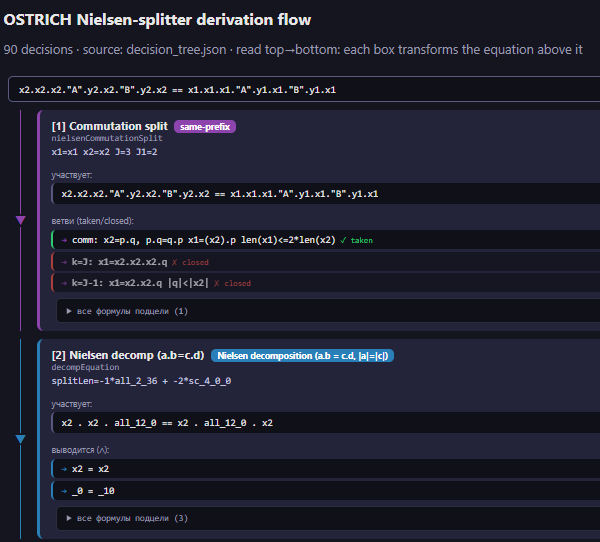
\includegraphics[height=0.46\textheight,keepaspectratio]{unsat_tree_html.png}\\[2pt]
      {\scriptsize Интерактивный HTML-вид узлов}
    \end{column}
    \begin{column}{0.58\textwidth}
      \centering
      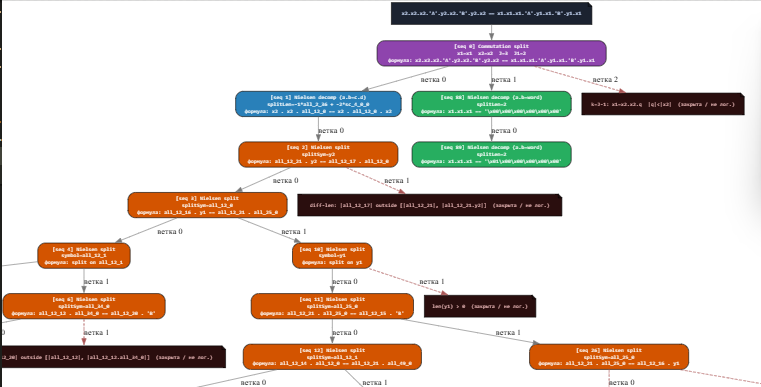
\includegraphics[width=\linewidth,keepaspectratio]{unsat_tree_graph.png}\\[2pt]
      {\scriptsize Граф потока вывода (Graphviz)}
    \end{column}
  \end{columns}
\end{frame}

% =====================================================================
\begin{frame}{Экспериментальная проверка}
  \begin{block}{Эвристики (вне решателя)}
    На наборе из \textbf{118 шаблонов} мгновенно разрешают \textbf{77\,\%} задач,
    \textbf{без единого ложного срабатывания}; медиана $<1$ мс.
  \end{block}

  \begin{block}{Решатель Ostrich vs. Z3}
    \begin{itemize}\setlength{\itemsep}{6pt}
      \item в среднем в \textbf{2,7 раза} быстрее Z3 (на общих задачах);
      \item на $x A x B y C y x$ --- до \textbf{1200 раз}: $151\,\text{с}\to 0{,}12\,\text{с}$;
      \item классы коммутации разрешили \textbf{2} ранее зависавшие задачи.
    \end{itemize}
  \end{block}

  \smallskip
  \centering\small\emph{Компоненты взаимодополняемы.}
\end{frame}

% =====================================================================
\begin{frame}{Ограничения и выводы}
  \begin{alertblock}{Ограничения}
    \footnotesize
    Выявлены непересекающиеся «слепые зоны» обоих алгоритмов --- это обосновывает
    применение специализированных эвристик лишь для узких классов задач.
    Классы коммутации \emph{не устраняют} бесконечное ветвление, а лишь упрощают
    прохождение части ветвей: даже на коммутативных классах возможны бесконечные циклы.
  \end{alertblock}

  \begin{block}{Выводы}
    \footnotesize
    Существенно расширена база однозначных и нетривиально неоднозначных образцов.
    Дальнейшее направление --- адаптация эвристик (рассчитанных на высокую кратность
    переменных и специфические константы) к \textbf{большему числу переменных} и
    константам в виде \textbf{перекрывающихся слов}.
  \end{block}
\end{frame}

% =====================================================================
\begin{frame}[plain]
  \centering
  \vfill
  {\Large Спасибо за внимание!}\\[1em]
  {\normalsize Готов ответить на вопросы.}
  \vfill
\end{frame}

\end{document}
